\documentclass[a4paper,10pt]{article}
\usepackage[utf8x]{inputenc}
\usepackage{graphicx}
\usepackage{color}
\usepackage{hyperref}
\usepackage[hmargin=3cm,vmargin=2.5cm]{geometry}
\usepackage{nameref}
%\usepackage{ulem}

% Meta data
\hypersetup {
    bookmarks=true,         % show bookmarks bar?
    unicode=false,          % non-Latin characters in Acrobats bookmarks
    pdftoolbar=true,        % show Acrobat's toolbar?
    pdfmenubar=true,        % show Acrobat's menu?
    pdffitwindow=false,     % window fit to page when opened
    pdfstartview={FitH},    % fits the width of the page to the window
    pdftitle={or-tools user's manual},    % title
    pdfauthor={Google},     % author
    pdfsubject={User's manual for the Google or-tools library},   % subject of the document
    pdfcreator={Google},   % creator of the document
    pdfproducer={Google}, % producer of the document
    pdfkeywords={or-tools} {open source} {constraint programming} {operations research}, % list of keywords
    %pdfnewwindow=true,      % links in new window
    colorlinks=true,       % false: boxed links; true: colored links
    linkcolor=blue,          % color of internal links
    citecolor=green,        % color of links to bibliography
    filecolor=magenta,      % color of file links
    urlcolor=cyan           % color of external links
}

\newcommand{\code}[1]{\texttt{#1}}
\DeclareRobustCommand{\hsout}[1]{\texorpdfstring{\sout{#1}}{#1}}

\newcommand{\gservers}{{\bf Google servers}}
\newcommand{\lhome}{{\bf Local home}}
\newcommand{\dhub}{{\bf Documentation hub}}

\setlength{\parindent}{0pt}


%opening
\title{How to generate the documentation for the or-tools library}
\author{Nikolaj van Omme\footnote{You can reach me at ortools.doc@gmail.com (or ask Laurent on how to reach me) if you need some help. ;-) }}
\date{\today}

\begin{document}

\maketitle

\begin{abstract}
This little document explains how to generate and upload all the documentation for the Google or-tools library. This document doesn't explain how to write the documentation i.e. how to use of \emph{Sphinx}, \emph{Jinja2}, \emph{html}, \emph{css}, etc., only how to generate the output files once
the documentation is written and how to upload the output files on the Google servers. All the scripts are written in Python and must be called in the correct sequence.\\
\begin{center}\textcolor{red}{Only tested under Linux.}\end{center}
\begin{center}\textcolor{red}{THIS INTERNAL DOCUMENT IS ONLY HELPFULL IF YOU WANT TO GENERATE THE DOCUMENTATION!}\footnote{You can get your local copy of the documentation and generate it if you want but there is no reason to do so as all the generated documentation is already available on the Google servers.}\\
\vspace{0.5cm}
\textcolor{red}{AS OF MAY 23, 2013, THIS DOCUMENT ACCURATELY DESCRIBES THE DOCUMENTATION GENERATION PROCESS.}\\
\vspace{0.2cm}
\textcolor{red}{Please update this document if you change anything to the documentation generation process.}
\end{center}

The documentation and the process to generate the or-tools library's documentation was designed with the or-tools people in mind. As such, the whole generation process isn't bullet-proof nor idiot-proof. In agreement with Laurent Perron, some tools were disregarded.\\

The contract only permitted to deal with a first version of the manual with the accompanying C++ code and the documentation HUB. The FAQ, slides and other documentation haven't been done~\ldots yet. In particular, the C++ code hasn't been translated into other languages.\\

This document itself is written in~\LaTeX\ and generated with~PDF\LaTeX.

\end{abstract}

\setcounter{tocdepth}{2}
\tableofcontents


%***************************************************************************************
\section{Preminilaries}
%***************************************************************************************
We quickly describe the involved directories and files.

%######################
\subsection{Vocabulary}
%######################

To avoid misunderstanding, let's agree on some wordings.

\begin{description}
 \item[Source/Code file] A file in wich you write the documentation. It can be restructuredText (.rst), \LaTeX\ (.tex) or text (.txt, .css, html, \ldots)\footnote{Basically, \emph{all} source files are text files.}. Some files are at the same time source and output files.
 \item[Output file] A file that will be published on the server side, including html files, images, etc. Some files are at the same time source and output files.
 \item[\lhome] The computer you use to write the documentation.
\item[Root directory] The local directory in your \lhome\ that contains locally all the files to generate the documentation. It is your workspace to generate the documentation.
 \item[\gservers] The servers where the documentation is publicly accessible from the Internet.
 \item[\dhub] A central html page from which all the documentation is accessible except the downloadable files. The url is:\\
 \href{http://or-tools.googlecode.com/svn/trunk/documentation/documentation\_hub.html}{http://or-tools.googlecode.com/svn/trunk/documentation/documentation\_hub.html}.
\end{description}

%######################
\subsection{Directories}
%######################

There are {\bf seven} main directories (illustrated on Figure~\ref{pic_directories} page~\pageref{pic_directories}).\\

{\bf Four} on the \lhome\ side:

\begin{description}
 \item[\code{SOURCES}] This local directory contains the sources files, the scripts files and some configuration files. This directory is a local copy of the the directory \code{doc\_sources}.
 \item[\code{BUILD}] This local directory contains all the automatically generated output files.\\
\hspace{2cm}{\bf Exceptions:} \code{HUB} (is build inside its source directory).
 \item[\code{DEPLOY}]  This local directory contains all the generated output files (automatically or by hand). It is not a local copy of the \code{trunk/documentation} directory as the directory structure is slightly different. We use it essentially for testing purpose. Consider this directory as a buffer between \code{BUILD} and~\code{DOCUMENTATION}. This buffer is 
also handy is the documentation is created and generated concurrently.
 \item[\code{DOCUMENTATION}] The real thing, i.e. the documentation you can access from the documentation hub. This local directory is a local copy of the \code{trunk/documentation} directory. Actually, it is more the opposite: \code{svn/trunk/documentation} is a copy of your local directory \code{DOCUMENTATION} as we push (commit) the generated documentation on the Google servers without pulling (updating) it.
\end{description}

and {\bf three} on the \gservers\ side:

\begin{description}
 \item[\code{svn/doc\_sources}] A server directory containing the sources files of the documentation. All the files you need to generate the documentation are stored in this directory. The full url is~\href{http://or-tools.googlecode.com/svn/doc\_sources}{http://or-tools.googlecode.com/svn/doc\_sources}.
 \item[\code{files}] A server directory containing the downloadable files. The full url is~\href{http://or-tools.googlecode.com/files}{http://or-tools.googlecode.com/files}. Note that you don't have public access to the directory, only to the files stored in it.
 \item[\code{svn/trunk/documentation}] A server directory with the or-tools library's documentation (except for the downloadable files). The full url is~\href{http://or-tools.googlecode.com/svn/trunk/documentation}{http://or-tools.googlecode.com/svn/trunk/documentation}.
\end{description}



%######################
\subsection{The \code{SOURCES} directory}
\label{doc_content}
%######################

The documentation is explained on the \dhub.\\

The local directory \code{SOURCES} contains the following files:

\begin{description}
 \item[\code{current\_version.txt}] Text file with the actual release number (xx.yy.zz), i.e. the release number of the next documentation you will upload. It is automatically updated after a new release is uploaded but you can manually update it
if necessary.
 \item[\code{global.rst}] Rst file with global variables.
 \item[\code{README.txt}] You know~\ldots the file you never read but really should read...
 \item[\code{TODO.txt}] What we plan for the future.
\end{description}

The local directory \code{SOURCES} contains the following directories:

\begin{description}
 \item[\code{doc}] The doc of the doc, i.e. the \LaTeX\ files to generate this document.
 \item[\code{FAQ}] Source files for the Frequently Asked Questions. The FAQ is generated by Sphinx. Needs to be rewritten and completed.
 \item[\code{HUB}] Sources files for the documentation hub. Written by hand but with the help of the Python \code{generate\_hub.py} script.
\item[\code{images}] Interesting images to use somewhere else. Kept here meanwhile.
 \item[\code{internals}] Internal files for the scripts. You shouldn't change anything here.
 \item[\code{LABS}] Exercises. Needs to be written.
\item[\code{LICENSES}] Different licenses. They are all regrouped in one place to easier update them as needed.
\item[\code{MANUAL}] The user's manual directory.
\item[\code{scripts}] Several Python scripts used throughout the or-tools documentation project.
\item[\code{SLIDES}] Tentative try to generate slides for the documentation. Has to be (re)written and a new approach with pygment is needed.
\item[\code{sphinxortools}] Tentative or-tools Sphinx extension. Abandonned after too many hair pulled out (Sphinx bugs).
Another avenue would be to use pre- and post-processing tools currently not recommended by Laurent. Because of 
numerous Sphinx (last version used: 1.1.3) bugs, you need to duplicate lots of texts, tags and tables in the source files.
\item[\code{TUTORIALS}] C++ code and hopefully other languages one day.
\end{description}



%***************************************************************************************
\section{How to Install the documentation sources and the needed tools}
%***************************************************************************************
\label{installation}

We describe here how to do a fesh installation of the sources to generate the documentation.

%######################
\subsection{Local directories and copies}
%######################

First, you need to setup your {\bf Local Root} directory as your working directory. Inside this directory, create the following directories:
\begin{itemize}
\item \code{SOURCES}
\item \code{BUILD}
\item \code{DOCUMENTATION}
\item \code{DEPLOY}
\end{itemize}

\code{SOURCES} and \code{DOCUMENTATION} are svn copies of \code{svn/doc\_sources} and~\code{svn/trunk/documentation} so you have to create them with~\code{svn}:\\

\code{svn checkout https://or-tools.googlecode.com/svn/doc\_source SOURCES --username me}\\

\code{svn checkout https://or-tools.googlecode.com/svn/trunk/documentation DOCUMENTATION --username me}\\

and type your \emph{GoogleCode.com Password} when prompted.\\

\code{BUILD} and~\code{DEPLOY} have to be manually created.\\

You also have to manually create:

\begin{itemize}
\item \code{DEPLOY/UPLOAD/manual}: To hold the generated manuels in pdf and epub formats.
\item \code{labs}, \code{tutorials} and~\code{reference\_manual}: these are copies of the corresponding directories in~\code{DOCUMENTATION}. The idea is to generate their content with~\code{generate\_*.py} and~\code{deploy\_*.py} scripts but this has to be done. For the moment, simply copy the directories. You don't need to copy~\code{reference\_manual} as a simple soft link will do.
\end{itemize}

%######################
\subsection{The~\code{config.ini} file}
%######################

Copy the~\code{config.ini} file from the \code{SOURCES/scripts} directory into your {\bf Local Root} directory. and fill in 
the first lines:

\begin{verbatim}
# Configuration file for the or-tools documentation project.
# All keys MUST be in lowercase.
[root]
dir = 

project = or-tools

[ortools]

dir = 

[personal]
password = 
username = 
\end{verbatim}

For instance, in my configuration:

\begin{itemize}
\item \code{dir = /mnt/data/RESEARCH/GOOGLE/OR\_TOOLS\_DOC}
\item \code{dir = /mnt/data/or-tools-read-only}
\end{itemize}

%######################
\subsection{External libraries and tools}
%######################

The following list details all the libraries and tools that you need to generate the documentation. Most of them are written in Python.

\begin{description}
 \item[Sphinx] This is the main library. It transforms \verb+restucturedText+ into plenty of other formats. The latest version the better. \code{Sphinx} is quite buggy but produces beautiful documents. The website can be found here:

\href{http://sphinx-doc.org/}{http://sphinx-doc.org/}

Some \code{Sphinx} extensions are used (or are planned to be used one day...):
 \begin{description}
\item[sphinx.ext.pngmath] Instead of using \code{MathJax}, we transform the formulas into \code{png}. The \code{MathJax} server is often too busy...
\item[sphinx.ext.ifconfig] To create different versions of the documentation (A4/USLetter, final/draft, \ldots).
\item[sphinxortools.ortools] Homemade extension that~\ldots doesn't work and is abandonned.
\item[sphinxcontrib.doxylink] No used yet. To create external links with the documentation generated by Doxygen.
\end{description}

\item[Jinja2] Jinja2 is a templating language for Python (used to generate the HTML code), The website can be found here:

\href{http://jinja.pocoo.org/}{http://jinja.pocoo.org/}

 \item[\LaTeX] To generate the pdf version of the manual, we use \LaTeX{} and \verb+pdflatex+ (and of course, the classical \verb+makeindex+/\verb+mkindex+, \verb+bibtex+, \ldots). \TeX Live is perfect.

\item[Xfig] To generate the pictures.

\item[fig2xxx] To convert \code{fig} files to \code{pdf}, \code{png} and \code{ps} when needed.

\item[ImageMagic] Very handy library to transform images.

 \end{description}

We use also Python (2.7), make, html, css, ...

%######################
\subsection{Scripts and first run}
%######################

By now, you should have a copy of \code{svn/doc\_sources} in \code{SOURCES}, a copy of~\code{svn/trunk/documentation} in~\code{DOCUMENTATION} and local copies of \code{labs}, \code{tutorials} and~\code{reference\_manual}.\\

The first run isn't different from a usual documentation update. See section~\ref{work_flow}.

%***************************************************************************************
\section{How to generate the manual}
%***************************************************************************************

We describe here how to generate the manual. The other parts of the documentation are generated in a similar fashion.
If you don't find a specific script in a subdirectory, it means that this script is not needed for that part of the  documentation.

%######################
\subsection{Work flow}
\label{work_flow}
%######################

The whole process is divided in 9~steps\footnote{Once you get used to the documentation generation, you will be able to skip some of the steps (when you don't need to update the whole documentation tree) and to only use the specific manual commands you need.}. Most of the steps are automated by Python scripts. These scripts need to be called in sequence. In each of the subdirectories of the directory~\code{SOURCES} (see section~\ref{doc_content}), you will find the corresponding Python scripts if needed.\\


\begin{figure}[h]
   \centering
   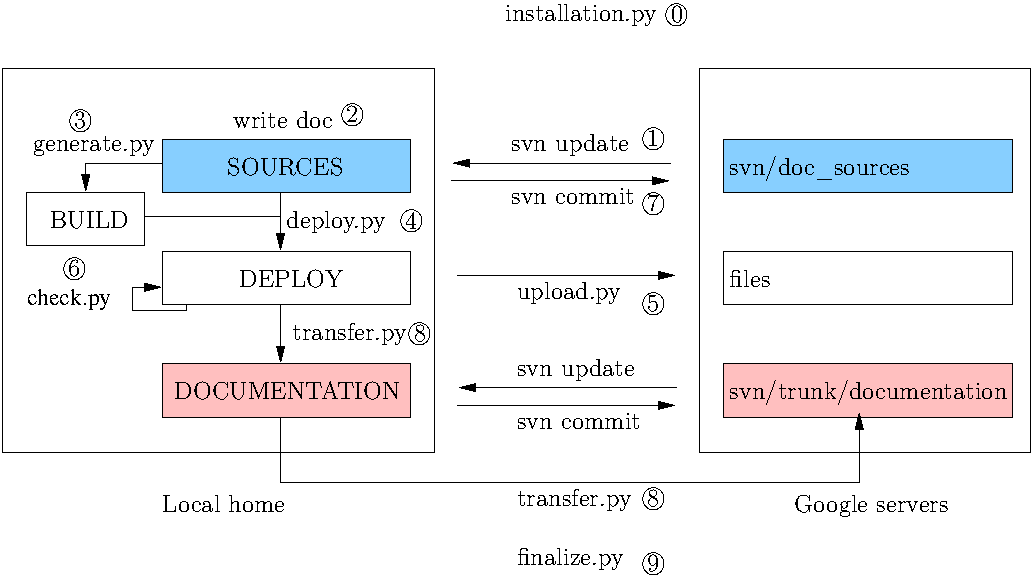
\includegraphics[scale=0.8]{images/directories.pdf}
   \caption{figure}{The six main directories and the scripts/commands to move the files between them. The base url for the Google Servers is~\href{http://or-tools.googlecode.com/}{http://or-tools.googlecode.com/}. The directories colored in the same color are svn copies of each other (white is not considered as a color).}\label{pic_directories}
 \end{figure}

\begin{description}
 \item[Step \raisebox{.3pt}{\textcircled{\raisebox{-.9pt} {1}}}] {\bf Update the source code:} (script: none)\\Update your local copy of the documentation via svn: \code{svn update}.
 \item[Step \raisebox{.3pt}{\textcircled{\raisebox{-.9pt} {2}}}] {\bf Write the documentation:} (script: none)\\Let your talent speak!

 \item[Step \raisebox{.3pt}{\textcircled{\raisebox{-.9pt} {3}}}] {\bf Generate the documentation:} (script: \code{generate\_xxx.py})\\Generate automatically the documentation. You will find the generated documentation
in the \code{BUILD}~directory. For the moment, only the manual (subdirectory~\code{MANUAL}) and the FAQ (subdirectory~\code{FAQ}) are automatically generated. If you are not uploading a new release on the~\gservers, you 
don't need to use this script: Sphinx provides a handy~\code{Makefile}.\\~\\
The~\dhub\ is parlty generated automatically, partly generated by hand.

 \item[Step \raisebox{.3pt}{\textcircled{\raisebox{-.9pt} {4}}}] {\bf Deploy the documentation:} (script: \code{deploy\_xxx.py})\\Copy locally the output files in the directory~\code{DEPLOY}. This directory is used to test
the documentation and try new things without messing with the svn directory.

\item[Step \raisebox{.3pt}{\textcircled{\raisebox{-.9pt} {5}}}] {\bf Upload the documentation:} (script: \code{upload\_xxx.py})\\Before you can check the documentation in the \code{DEPLOY}~directory, and if you want to test the download links, you have to upload the downloadable files. The \code{upload\_xxx.py}~script will be stuck if you try to upload a file that is already uploaded (based on the filename). If you want to update a downloadable file, you first have to delete the file from the Google servers. For the moment, this action has to be done manually through web user interface. If you know how to do it with a script, we are interested!

 \item[Step \raisebox{.3pt}{\textcircled{\raisebox{-.9pt} {6}}}] {\bf Check the documentation:} (script: \code{check.py} in the~\code{scripts} directory)\\Check the documentation. As of May 23 2013, the \code{check.py}~script only checks internal links for the manual (via the script~\code{check\_internal\_refs.py}). The rest is a manual (and important!) process 
(Sphinx does provide some handy tools).

 \item[Step \raisebox{.3pt}{\textcircled{\raisebox{-.9pt} {7}}}] {\bf Update the documentation source:} (script: none)\\If you're happy with the new documentation, commit your changes on the Google solvers. This step can be completed after step~\raisebox{.3pt}{\textcircled{\raisebox{-.9pt} {9}}}.

 \item[Step \raisebox{.3pt}{\textcircled{\raisebox{-.9pt} {8}}}] {\bf Upload the documentation:} (script: \code{transfer.py} in the~\code{scripts} directory)\\Push (commit) the documentation on the Google servers. Prefer to use the \code{transfer.py}~script over the svn commands as it completes all required tasks in a single procedure. As of 23 May 2013, \code{transfer.py} only calls the~\code{svn\_documentation\_commit.py} script
that - despite its name - only commits the html version of the manual. You can roll a dry run with the~\code{compare\_deploy\_vs\_documentation.py} than will create the~\code{added.txt}, \code{changed.txt} and~\code{deleted.txt} files with explanatory filenames. It's best to use this script before commiting~\emph{atrocities}.

 \item[Step \raisebox{.3pt}{\textcircled{\raisebox{-.9pt} {9}}}] {\bf Prepare the next release of the documentation:} (script: \code{finalize.py} in the~\code{scripts} directory)\\As of May 23 2013, \code{finalize.py} only calls the~\code{versions.py} that update the version number for the next release.\\

The documentation has a release number (xx.yy.zz). It is used internally by the scripts to check the validity of the documentation. The \code{versions.py}~script will copy the old number and update the new number (for instance, from 4.5.11 to 4.5.12 by default). You MUST use this script after step~\raisebox{.3pt}{\textcircled{\raisebox{-.9pt} {8}}}. If you want to update the release number to a higher release number, edit manually the file~\code{current\_version.txt} in the~\code{SOURCES} directory WITHOUT calling this script.
\end{description}

%######################
\subsection{Preferred use}
%######################

These scripts are not bullet-proof nor idiot-proof (and can be easely improved). I strongly suggest that the source files always match the documentation files in:

\begin{center}
\href{http://or-tools.googlecode.com/svn/trunk/documentation}{http://or-tools.googlecode.com/svn/trunk/documentation}.
\end{center} 

Once you have finished steps \raisebox{.5pt}{\textcircled{\raisebox{-.9pt} {1}}} - \raisebox{.5pt}{\textcircled{\raisebox{-.9pt} {6}}}, commit your changes on the Google solvers (step \raisebox{.5pt}{\textcircled{\raisebox{-.9pt} {7}}}). If there is a conflict, start the whole process again later with the updated documentation sources. One easy way to ensure the consistency between the sources and the documentation is to delegate the upload and commitment of the documentation (steps \raisebox{.5pt}{\textcircled{\raisebox{-.9pt} {8}}} - \raisebox{.5pt}{\textcircled{\raisebox{-.9pt} {{9}}}}) to one single person (or to redesign the whole process ;-) ). This design ask for some discipline but I think it is manageable among Googlers.





%######################
\subsection{Different versions}
\label{manual_different_version}
%######################

The manual exists in several versions:

\begin{description}
\item[\code{a4}] European~\code{a4} format.
\item[\code{letter}] American~\code{USLetter} format.
\item[\code{epub}] \code{epub} generation.
\item[\code{latexpdf}] \code{pdf} generation.
\item[\code{draft}] \code{draft} release.
\item[\code{final}]  \code{final} release.
\end{description}

The very handy~\code{..  only::} directive allows to target a specific version of the manual. For instance, if you don't want
to publish some material, use:
\begin{center}
\code{..	only:: draft}
\end{center}

You can use the~\code{convert\_draft\_to\_final.py} script located in the~\code{scripts} directory to get rid of the~\code{..	only:: draft} directives.

%***************************************************************************************
\section{\dhub}
%***************************************************************************************

Some explanation about the generation of the~\dhub.
\subsection{The change files/directory}

\begin{description}
 \item[changes.txt] This is where you write what changed since the last upload of the documentation. This file is automatically inserted in \verb+documentation_hub.html+ so be carefull! ;-) Lines starting with \verb+#+ are comments that are not written in the html file. Don't add the version, this is done automatically. Note that this file is not automatically updated. You are responsible for its content.
 \item[changes\_list.txt] This file is automatically updated with the content of \verb+changes.txt+.
 \item[changes] This directory contains copies of all the \verb+changes.txt+ files.
 \end{description}




%***************************************************************************************
\section{Gotchas}
%***************************************************************************************

Here we summarize some bugs, mistakes, difficulties, etc. When in doubt, you always can use the \code{restructuredText}
\code{raw} directive.

\begin{itemize}
\item The tables are really badly handled in Sphinx...
\item References are badly handled in Sphinx... You need to duplicate them in the source files if you want to generate the well-known \emph{see section~11.4.3} for instance in~\LaTeX\ generated documents. See next item.
  \item Capitalized letters in a~\code{rst} reference become lower letters and underscores ("\_") become dashes ("-") in the~\code{Sphinx} generated references. So for instance, if the reference in your~\code{rst} file \code{my\_file.rst} in the directory~\code{manual/my\_chapter/} is~\code{MyStrange\_referenceIa}, the~\code{Sphinx}~\LaTeX~reference will be~\code{manual/my\_chapter/my\_file:mystrange-referenceia}. 


 \item When in draft mode (see~\ref{manual_different_version}), the section numbers in the html pages are wrong. 
 \item \LaTeX\ slides files have to start with \code{\textbackslash documentclass\{\}} on the first line (required by \code{generate\_slides.py}).
\item Often, images and figures need to be duplicated: one version for the~\code{hmtl} and~\code{epub} manuals, one version for the~\LaTeX\ generated documents.
 \item Manual: the preface is copied once. This is necessary as Sphinx doesn't allow to differentiate between titles in \LaTeX\ and Sphinx.
 \item There is no automatic update between the Getting started page of the wiki and the one of the manual. If you change one, you have to change the other manually. 
 \item When you want to use class names in titles and want to talk about them in the plural, you have to add ~\verb+\s+, not just~\verb+s+:
  \begin{verbatim}
``SearchMonitor``\s
-------------------
  \end{verbatim}
\end{itemize}


\end{document}
